\documentclass[11pt]{article}
\usepackage{fontspec}
\setmainfont{Arial}
\setsansfont{Arial}
\setmonofont{Arial}
\usepackage[margin=1in]{geometry}
\usepackage{amsmath,amssymb}
\usepackage{graphicx}
\usepackage{adjustbox}
\usepackage{placeins}
\usepackage{booktabs}
\usepackage{multirow}
\usepackage{siunitx}
\usepackage{caption}
\usepackage{subcaption}
\usepackage{tikz}
\usetikzlibrary{arrows.meta,positioning,calc,fit,decorations.pathreplacing}
\usepackage[numbers,round]{natbib}
\usepackage[svgnames]{xcolor}
\usepackage{authblk}
\usepackage{microtype}
\usepackage{xurl}
\usepackage[hidelinks]{hyperref}

\captionsetup{font=small,labelfont=bf,skip=6pt}
\setlength{\parskip}{0.3em plus 0.1em minus 0.1em}
\setlength{\parindent}{0pt}

\newcommand{\panfig}[1]{\resizebox{\textwidth}{!}{\input{#1}}}
\newcommand{\panhalffig}[1]{\resizebox{0.98\linewidth}{!}{\input{#1}}}

\tikzset{every node/.append style={font=\sffamily\mdseries,text=black}}
\setlength{\emergencystretch}{2em}
\setlength{\floatsep}{10pt plus 2pt minus 2pt}
\setlength{\textfloatsep}{11pt plus 2pt minus 2pt}
\setlength{\intextsep}{10pt plus 2pt minus 2pt}
\renewcommand{\topfraction}{0.94}
\renewcommand{\bottomfraction}{0.9}
\renewcommand{\textfraction}{0.08}
\renewcommand{\floatpagefraction}{0.90}
\makeatletter
\setlength{\@fptop}{0pt}
\setlength{\@fpsep}{12pt}
\setlength{\@fpbot}{0pt plus 1fil}
\makeatother
\setcounter{topnumber}{4}
\setcounter{totalnumber}{6}
\clubpenalty=10000
\widowpenalty=10000
\displaywidowpenalty=10000

\graphicspath{{figures/}{standalone-assets/}{tikz/}{./}}
\hypersetup{pdftitle={Single-topic collapse in a within-cell attention topic model: an implementation and measurement case study},pdfauthor={Zeyu Fu}}

\title{\textbf{Single-topic collapse in a within-cell attention topic model:\\ an implementation and measurement case study}}
\author[1]{Zeyu Fu}
\affil[1]{State Key Laboratory of Trauma and Chemical Poisoning, Institute of Combined Injury,
Chongqing Engineering Research Center for Nanomedicine, College of Preventive Medicine,
Army Medical University, Chongqing, China\\
\texttt{fuzeyu09@gmail.com}}
\date{}

\begin{document}
\maketitle


\begin{abstract}
A topic allocation can lose almost all between-cell variation while remaining a valid probability vector. We examine this distinction in a small, non-flow-matching topic autoencoder whose attention layers operate over eight projected tokens within each cell. In archived Setty runs at concentration $\alpha=0.1$, all 450 held-out cells select the same dominant topic within each run, for three seeds at each of the 200-, 400-, and 1000-epoch caps. The dominant topic differs across seeds. Allocation perplexity is approximately one, while the exact zero printed by the legacy coherence scorer is a degeneracy sentinel, not a measured biological effect. The 1000-cap runs stop at 607, 492 and 536 epochs. Other backgrounds do not show uniform degeneracy. We distinguish this representation failure from graph reachability and prediction of computational Palantir branch probabilities, and withhold branch scores for degenerate allocations. A new twelve-arm, initialization- and schedule-matched concentration experiment completes 3200 updates per arm: low-concentration Setty collapse recurs on two of three seeds (exact 95\% binomial interval 0.094--0.992); the other seed and all Dentate runs fail strict collapse. Token and batch-context interventions check the implementation, not the scientific cause of collapse. The evidence identifies a configuration-specific failure; attention attribution requires an unrun parameter-matched MLP control and substantially more seeds.
\end{abstract}

\noindent\textbf{Scope of inference.} The matched low-concentration Setty strict-collapse frequency is $2/3$, with an exact seed-level 95\% binomial interval of 0.094--0.992. The token and batch-context probes are implementation checks; they cannot attribute collapse to attention. A parameter-matched MLP gate and a larger-seed phase diagram remain prospective.

\section{Introduction}
A representation can be mathematically valid while conveying almost no distinction between observations. This problem is especially easy to overlook when a model exports a normalized probability vector: every row can sum to one even when all rows assign nearly all their mass to the same component. Topic models define observations through mixtures over latent components~\cite{blei2003latent}, and neural variational constructions provide a practical way to fit related count models~\cite{srivastava2017autoencoding}. Their constraints specify the space of possible outputs, but do not ensure that a trained model uses that space informatively. Before interpreting topic allocations as cell programs, their variation across cells must therefore be examined directly.

Self-attention adds flexible interactions among learned representations, but its scientific interpretation depends on the objects that attend to one another. The transformer architecture introduced attention-based sequence processing~\cite{vaswani2017attention}; an application to expression counts need not use genes, cells, or biological pathways as its tokens. In the model examined here, each cell's full feature vector passes through eight learned projections, producing eight within-cell tokens. Those tokens interact through two attention layers and a pooling query before parameterizing a topic allocation. The model is therefore neither a cross-cell attention system nor a pretrained gene-language model. Stating the tensor axes and projection construction is necessary before asking what a failure says about attention.

The prior regularizer presents another interpretive boundary. A low concentration parameter may encourage sparse topic proportions, but sparsity within each cell is distinct from diversity between cells. Distinct cells can occupy different simplex corners, or occupy the same corner with almost no between-cell information. Perplexity near one cannot distinguish these possibilities; coordinate range, argmax occupancy and native distances supply complementary checks. We call the latter behavior allocation collapse. Posterior collapse in variational inference instead concerns a posterior approaching its prior or failing to use latent variables~\cite{lucas2019collapse}. Constancy of $\operatorname{softmax}(\mu)$ alone does not establish either posterior equality or the behavior of the learned variance.

Distance-based summaries can become misleading near this boundary. An allocation-coherence ratio compares similarity among graph neighbors with similarity among arbitrary cells. When every allocation is nearly identical, both quantities approach zero and their ratio becomes numerically unstable or undefined. A software sentinel returned for this condition is a reporting convention, not a biological measurement. Graph reachability can remain nontrivial because neighbor construction, ties, and graph thresholds operate on a different object. A repeated scalar graph fraction also need not identify the same severed edges. Reliable interpretation requires the status of the native representation, the estimator's denominator, and the graph's identity to remain separate observations.

Low-dimensional visualization creates a further opportunity for confusion. UMAP~\cite{mcinnes2018umap} produces a fitted two-dimensional layout from a representation, and a visually structured layout does not establish that the underlying allocation contains the intended biological information. Label-neighbor purity in that layout has its own definition, including how self-neighbors are excluded. Correcting a neighbor-selection rule can change the displayed score without changing any coordinates or training outcome. Similarly, agreement with Palantir branch probabilities~\cite{setty2019palantir} describes a computational annotation rather than experimentally observed fate. A degenerate allocation should not acquire apparent credibility because a separate visualization or graph summary happens to look plausible.

To determine whether an apparent failure is transient, comparisons must account for optimization exposure. An observation at one short training cap could reflect an unfinished fit, but increasing the cap does not create equal exposure when different runs stop early. Historical endpoints are useful records of actual behavior, provided completed epochs are reported and the same endpoint is not counted repeatedly as a new replication. A new controlled concentration comparison can strengthen this evidence by matching the autoencoder initialization, batch sequence, stochastic draws, and number of optimizer updates. Direct interventions on the trained token tensor can then test whether the implemented pathway responds to token content or inadvertently mixes information between cells.

This study examines an attention-based count topic model across four public expression backgrounds, with particular focus on low-concentration hematopoietic allocations. Historical native arrays permit direct assessment of allocation variation alongside graph and visualization readouts. A new matched concentration experiment in hematopoietic and dentate data tests the sensitivity of native allocations under complete fixed training budgets. Trained-state interventions compare token permutation, token homogenization, token duplication, and changes to the other cells in a batch. These interventions have distinct roles: invariance controls test the computation's intended axes, while content changes test local sensitivity. The objective is a self-contained account of allocation behavior and its measurable boundaries, without inferring that attention architectures generally collapse or that an informative allocation automatically identifies a biological lineage.

\section{Materials and Methods}
Figure~\ref{fig:arch} locates the within-cell attention tensor, native allocation and interventions before specifying their objective. The architecture identifies the measured pathway without attributing collapse to attention alone.
\begin{figure}[!htbp]
\centering
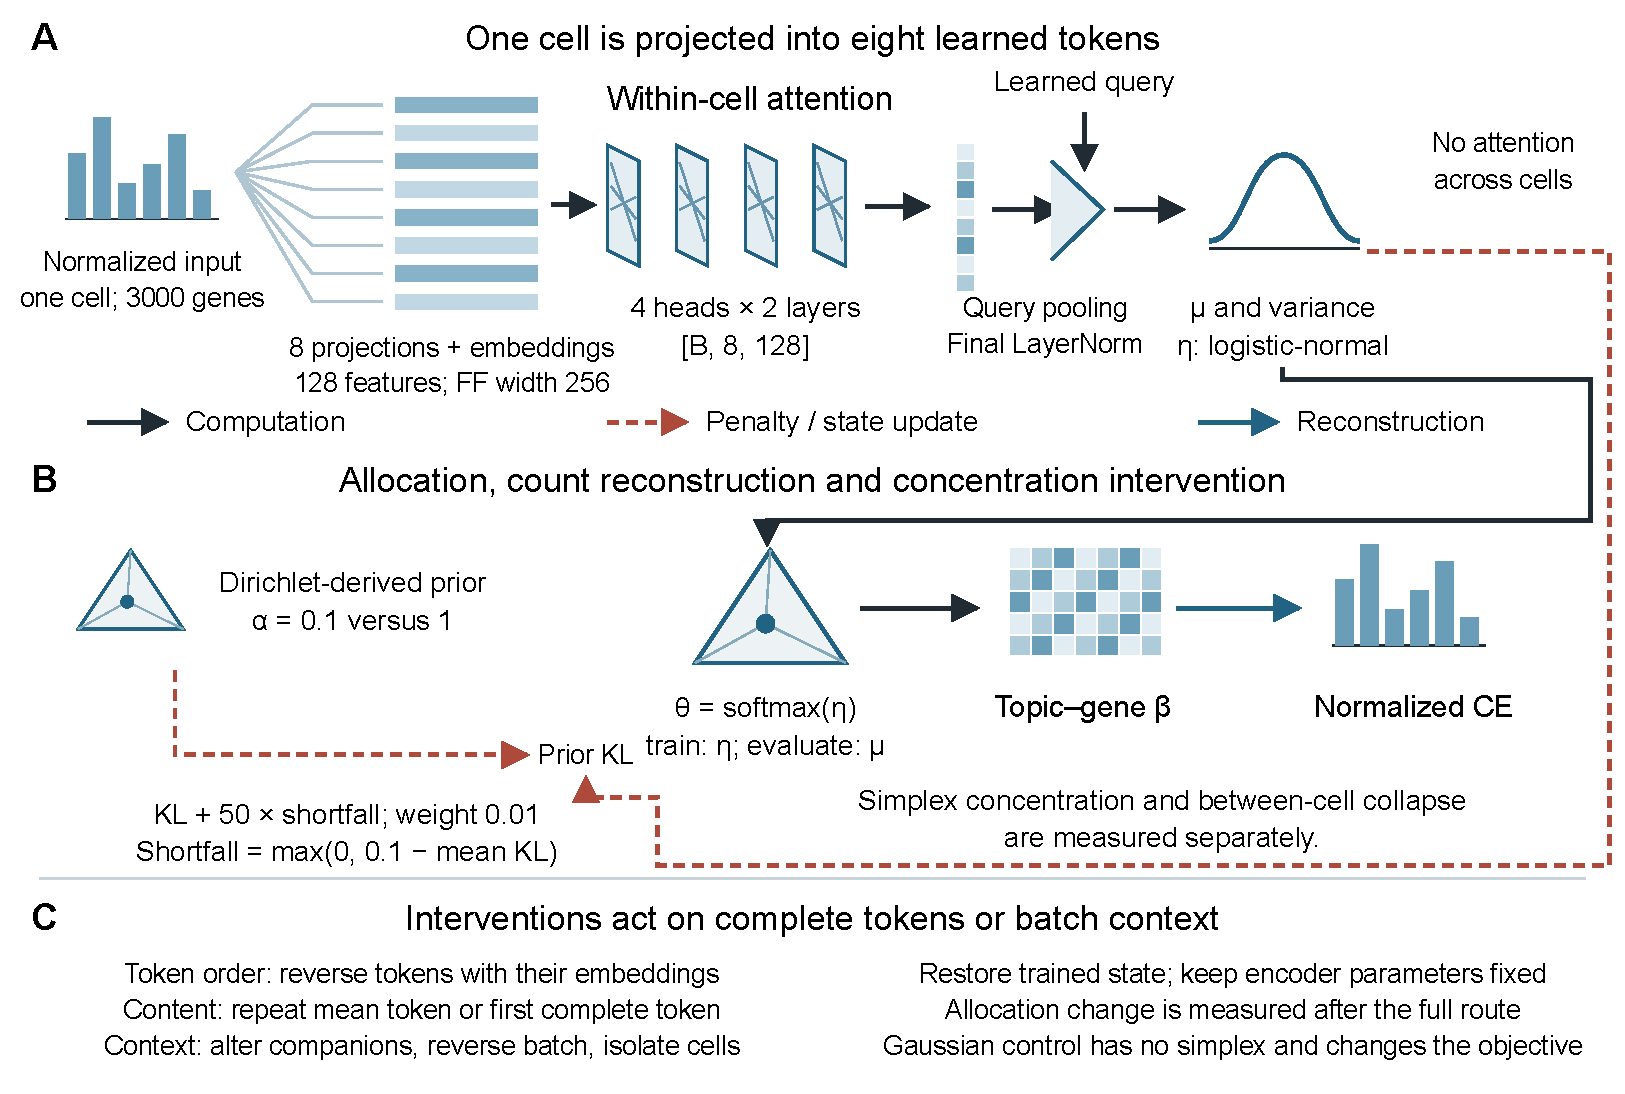
\includegraphics[width=\textwidth]{figures/architecture.pdf}
\caption{\textbf{Within-cell attention, allocation and intervention routes.} A: eight independent full-expression projections produce $[B,8,128]$ tokens; two four-head attention layers and learned-query pooling parameterize ten logit means and variances. B: sampled logits give a simplex and topic--gene reconstruction; the concentration-dependent KL has weight 0.01 and a custom $50\max(0,0.1-\bar d_k)$ shortfall term (Eq.~\ref{eq:topic-objective}). Evaluation uses $\operatorname{softmax}(\mu)$. C: token and batch-context probes act on restored endpoints. Shapes denote computational objects. Tokens are not named genes, attention is within-cell, and the Gaussian comparator changes multiple model factors.}
\label{fig:arch}
\end{figure}
\subsection{Within-cell attention and the optimized objective}
A normalized expression vector with $G=3000$ features is mapped through eight separate Linear--LayerNorm--GELU projections to width 128, then added to learned token embeddings. Two transformer layers, each with four 32-dimensional heads and feedforward width 256, act on $[B,8,128]$. A learned query pools the tokens by cross-attention, followed by LayerNorm and two $128\to10$ output heads. This query pooling is related to the permutation-invariant construction of Set Transformer~\cite{lee2019set}; it does not make the input genes exchangeable. Dropout is zero. The posterior in logit coordinates is $q(\eta\mid x)=\mathcal N(\mu(x),\operatorname{diag}v(x))$, with $v=\operatorname{softplus}(h_v)+10^{-4}$. One reparameterized draw per cell and update~\cite{kingma2014auto} gives $\eta=\mu+\sqrt v\odot\epsilon$, $\epsilon\sim\mathcal N(0,I)$, and $\theta=\operatorname{softmax}(\eta)$. Evaluation exports $\operatorname{softmax}(\mu)$, not a Monte Carlo posterior average.

For trainable topic--gene logits $b\in\mathbb R^{10\times G}$, $\beta_{kg}=\operatorname{softmax}(b_{k\cdot})_g$ and $p_{ig}\simeq\sum_k\theta_{ik}\beta_{kg}$. The shipped ``multinomial'' reconstruction actually uses cell-normalized counts $\tilde x_{ig}=x_{ig}/(\sum_gx_{ig}+\varepsilon)$:
\begin{equation}
 \mathcal L_{\rm rec}=-\frac1B\sum_{i=1}^B\sum_{g=1}^G
 \tilde x_{ig}\log(p_{ig}+\varepsilon),\qquad \varepsilon=10^{-10}.
\end{equation}
The decoder adds $\varepsilon$ inside $\log\theta$ and bounds reconstructed probabilities to $[\varepsilon,1-\varepsilon]$ before this loss. Thus the reconstruction is cross-entropy in nats per normalized cell, rather than a total-count-weighted multinomial log likelihood.

For concentration vector $\alpha$, the implemented diagonal logit-space prior has
\begin{equation}
 m_k=\psi(\alpha_k)-\frac1K\sum_j\psi(\alpha_j),\qquad
 s_k^2=\max\left\{10^{-6},\psi_1(\alpha_k)-\frac1{K^2}\sum_j\psi_1(\alpha_j)\right\}.
\end{equation}
Here $K=10$; under the symmetric concentrations tested, $m_k=0$ and $s_k^2=(1-1/K)\psi_1(\alpha)$. This is the code's diagonal surrogate, not an exact Dirichlet posterior or full centered-log-ratio covariance. With $\bar d_k=B^{-1}\sum_i d_{ik}$,
\begin{align}
 d_{ik}&=\frac12\left[\frac{v_{ik}+(\mu_{ik}-m_k)^2}{s_k^2+\varepsilon}-1
       +\log(s_k^2+\varepsilon)-\log(v_{ik}+\varepsilon)\right],\\
 \mathcal L&=\mathcal L_{\rm rec}+0.01\sum_{k=1}^{10}
       \left[\bar d_k+50\max(0,0.1-\bar d_k)\right].\label{eq:topic-objective}
\end{align}
The code calls this term ``free bits'', but conventional free bits uses a flat KL allowance~\cite{kingma2016iaf}. Here the batch-averaged per-coordinate shortfall is penalized linearly: away from the kink, its derivative with respect to $\bar d_k$ is $-49$ below 0.1 and $1$ above 0.1, before the 0.01 weight. It therefore pushes low KL upward rather than merely switching its penalty off. At $\alpha=1$ this regularizer remains active. Word-prior buffers do not enter the loss; there is no flow-matching stage.



\subsection{Backgrounds, split and optimization}
The backgrounds are Setty hematopoiesis~\cite{setty2019palantir}, dentate gyrus~\cite{hochgerner2018conserved}, pancreatic endocrinogenesis (Endo)~\cite{bastidas2019endocrinogenesis}, and human lung GSE130148~\cite{vieirabraga2019lung}. The lung accession contains fresh resected tissue from four patients, sampled from tumor-uninvolved regions; it is not a lung-development dataset despite the local filename. Historical preprocessing selects up to 3000 cells and 3000 genes before the split. Setty, dentate and lung use 2100/450/450 train/unused-validation/test cells; Endo uses 1771/379/381. These are within-file cell splits, not external cohorts or independent donors. Historical training uses physical batch size 128, AdamW learning rate and weight decay $10^{-3}$, gradient clipping at 10, and a training-loss patience of fifty epochs; caps are not necessarily completed epochs. A training seed is not a donor.

The 200-cap grid has 60 topic dose runs and 12 controls. It varies five concentrations across four backgrounds and three training seeds at $K=10$. Additional locks contain a Setty 400-cap comparison, a dedicated $\alpha=0.1$ 400-cap check, and 48 transformer runs at cap 1000.

AdamW uses decoupled weight decay~\cite{loshchilov2019decoupled}. Global parameter-gradient norm clipping at 10~\cite{pascanu2013difficulty} follows backpropagation and differs from the coordinate-KL transformation in Eq.~\ref{eq:topic-objective}. There is no AMP, accumulation or scheduler. The validation subset is unused and the endpoint is the final state, not a restored best checkpoint. We distinguish the cap from actual completed epochs and do not treat reused endpoints as new replications.

\subsection{Readouts and version boundaries}
The geometry reference is PCA-50 fitted to the held-out expression matrix in the historical audit. RAAG therefore measures alignment to a transductive expression reference. Palantir branch probabilities~\cite{setty2019palantir} are existing computed annotations in the same Setty object; five-fold $k$NN regression and distance correlation assess agreement with that proxy, not experimentally observed fates.

For native simplex rows, allocation coherence compares edge Jensen--Shannon divergence with a baseline over distinct cell pairs. The archived estimator samples this baseline; when it is at most $10^{-12}$, the legacy implementation returns zero and a degeneracy flag. A ratio is not interpretable under this condition. The revision displays exact distinct-pair coherence on archived native arrays and marks degenerate ratios n.q. in tables and plots. The old sampled estimates and zero sentinels remain in the immutable archives and explicit version mapping, rather than being silently relabeled.

UMAP~\cite{mcinnes2018umap} is an independent two-dimensional projection for each seed. The corrected purity calculation keeps every coordinate unchanged and recomputes label purity using the first 15 non-self neighbors. The old code had skipped the nearest neighbor after an API call that already excluded self; old purity values are superseded, not renamed.

\subsection{Matched concentration training}
The new experiment freezes Setty and Dentate input matrices, their historical 2100/450/450 split and normalized features. It trains seeds 0, 1 and 2 at $\alpha=0.1$ and 1, giving twelve arms, with the exact architecture and custom shortfall objective in Eq.~\ref{eq:topic-objective}. Within each pair the full autoencoder state is copied identically. Topic-prior buffers are derived separately from the two concentrations and hashed; the word-prior buffers are fixed at unit concentration and do not enter the implemented loss.

Each epoch uses the first 2048 indices of a newly generated permutation of the 2100 training cells, partitioned into sixteen physical batches of 128. NumPy seed $90000+s$ generates all 200 permutations and the 3200 per-step random seeds before either paired arm is fitted. Each arm resets the torch random seed at every step. AdamW uses learning rate and weight decay 0.001, gradient norm clipping at 10, no mixed precision, no scheduler, no accumulation and no early stopping. Every arm completes 3200 updates and 409600 presentations, for totals of 38400 and 4915200. Initial and last states, loss traces, schedules and hashes are retained. Native final allocations use deterministic $\mathrm{softmax}(\mu)$ on all 450 test cells. No best-state selection occurs.

Strict collapse is frozen as one occupied argmax topic together with maximum across-cell coordinate range at most $10^{-8}$. Mean row perplexity and exact distinct-pair Jensen--Shannon divergence are separate readouts; divergence at most $10^{-12}$ is flagged degenerate. Setty branch probability prediction is auxiliary: uniform 15-neighbor regression uses five shuffled folds with seed 42 and mean multi-output $R^2$. Degenerate allocations have no reported branch score. This new fold implementation and random schedule define a fresh experiment rather than an exact historical replay. All twelve outcomes are retained without significance testing.

\subsection{Token and batch-context probes on trained endpoints}
The probe restores each last state and uses the first 64 stored test cells. It extracts deterministic allocations in evaluation mode and training mode with dropout zero. A forward pre-hook on the actual transformer input acts after the eight learned projections and token embeddings, on the tensor $[64,8,128]$. Complete-token reversal moves each embedding with its token. Mean replacement repeats the per-cell average token eight times; duplication repeats the first complete token eight times. Encoder parameters and other computations remain fixed. The saved output includes each cell's allocation under every intervention, the maximum absolute coordinate change and the mean row $L_1$ change from the unmodified result.

For batch context, the first sixteen cells are focal. The remaining 48 normalized expression vectors are multiplied by ten while focal inputs remain fixed; a second control reverses batch order and restores it after evaluation; a third evaluates focal cells individually. The prespecified tolerance for permutation and batch invariance is $10^{-5}$ maximum absolute allocation change. These CPU-only probes use two numerical threads and zero optimizer updates. Content-change magnitudes are descriptive and are not tested against an optimized threshold. The mechanisms are tested in real trained states, not inferred from untrained behavior.

\subsection{Seed-level uncertainty and prospective gate}
For each fixed dataset--concentration cell, strict-collapse status is a Bernoulli outcome per training seed, not per held-out cell. Two-sided exact 95\% Clopper--Pearson intervals~\cite{clopper1934limits} invert the binomial tails, with endpoints $\operatorname{Beta}^{-1}(0.025;x,n-x+1)$ and $\operatorname{Beta}^{-1}(0.975;x+1,n-x)$ and boundary values zero or one for $x=0$ or $n$. The audit independently recomputes all twelve native arrays, verifies the flags and compares beta-quantile intervals with the saved binomial-inversion script. An exploratory range-threshold check at $10^{-10}$ and $10^{-6}$ supplements the frozen $10^{-8}$ cutoff without replacing it. Seed-deletion checks assess influence. The parameter-matched MLP and larger-seed phase diagram in the prospective freeze remain unexecuted.

\subsection{Geometry and allocation scoring definitions}
Reference and candidate Euclidean 15-neighbor graphs are symmetrized by union. The archived helper requests 16 neighbours and drops the first index, assuming it is self. Exact duplicate rows can violate that assumption and induce self-loops or row-order-sensitive ties. All twelve newly trained native arrays have 450 unique rows, no retained self-index and no exact distance tie at the 15-neighbour cutoff in the audit; this check does not validate the historical near-degenerate geometry against rounding or perturbation. The frozen scorer is retained. Reachability measures retention of connected unordered reference pairs. Edge survival averages reciprocal candidate shortest-path hop distance over reference edges, assigning zero to disconnected endpoints. Separation uses reference pairs at or above the 90th percentile of finite hops and tests whether candidate hops reach the candidate median; disconnected pairs count as separated. Native coherence is one minus mean edge Jensen--Shannon divergence divided by its exact mean over all distinct unordered pairs, in natural-log units. A denominator at most $10^{-12}$ is degenerate, and mean perplexity above $0.95K$ is near-uniform. Those cases are withheld from interpretable coherence summaries. Perplexity is exponential row entropy, independently reported even when coherence is undefined.

\section{Results}
\subsection{Concentration is not information retention}
Figure~\ref{fig:dose} and Table~\ref{tab:alpha} distinguish the concentration axis from coherence. Increasing $\alpha$ generally spreads allocations over more topics, but no common monotone biological benefit follows. Unreliable or degenerate branch readouts are omitted in Figure~\ref{fig:branch}; their absence must not be read as a zero prediction score.
\begin{figure}[htbp]
\centering
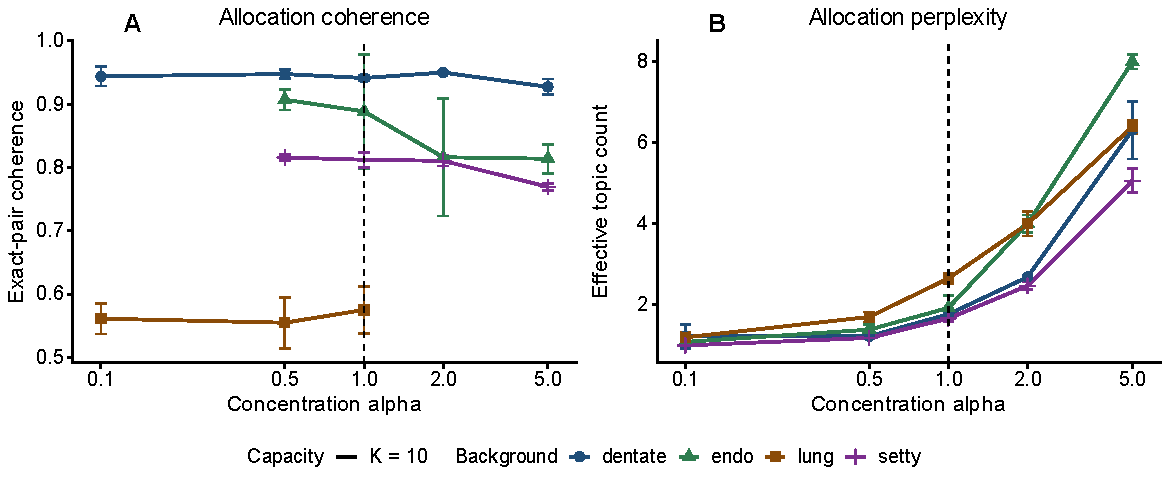
\includegraphics[width=\textwidth,height=0.72\textheight,keepaspectratio]{figures/topic-transformer_dose.pdf}
\caption{\textbf{Historical concentration grid at the 200-epoch cap, $K=10$.} A: exact-pair native-allocation coherence. B: mean row perplexity (effective topic count). Concentration is logarithmic; the dashed line marks $\alpha=1$. Color and shape identify backgrounds in the shared key. Points and bars are three-seed means and sample SD within fixed public-file splits; lines connect tested doses. Archived latents are unchanged. Unreliable ratios are omitted and marked n.q. in Table~\ref{tab:alpha}; they are not zeros. Seeds do not estimate donor uncertainty.}
\label{fig:dose}
\end{figure}
\begin{table}[htbp]
\centering
\caption{\textbf{Historical 200-cap allocation and Setty branch readouts.} Mean and seed SD are descriptive. n.q. denotes a readout rejected by the reliability rule. Setty $\alpha=0.1$ is degenerate; its coherence and branch scores are withheld rather than displaying the legacy zero sentinel. Perplexity near one indicates single-topic concentration, not an empty simplex.}
\label{tab:alpha}
\scriptsize
\setlength{\tabcolsep}{3.5pt}
\begin{tabular}{llccccc}
\toprule
Metric & Background & $\alpha=0.1$ & $\alpha=0.5$ & $\alpha=1$ & $\alpha=2$ & $\alpha=5$ \\
\midrule
\multirow{4}{*}{Allocation coherence} & dentate $K=10$ & 0.944 $\pm$ 0.015 & 0.947 $\pm$ 0.007 & 0.941 $\pm$ 0.005 & 0.950 $\pm$ 0.002 & 0.927 $\pm$ 0.013 \\
 & endo $K=10$ & \textit{n.q.} & 0.907 $\pm$ 0.016 & 0.888 $\pm$ 0.090 & 0.816 $\pm$ 0.093 & 0.814 $\pm$ 0.023 \\
 & lung $K=10$ & 0.561 $\pm$ 0.024 & 0.555 $\pm$ 0.040 & 0.575 $\pm$ 0.037 & \textit{n.q.} & \textit{n.q.} \\
 & setty $K=10$ & \textit{n.q.} & 0.816 $\pm$ 0.005 & 0.812 $\pm$ 0.012 & 0.810 $\pm$ 0.008 & 0.769 $\pm$ 0.005 \\
\midrule
\multirow{4}{*}{Allocation perplexity} & dentate $K=10$ & 1.223 $\pm$ 0.290 & 1.228 $\pm$ 0.046 & 1.769 $\pm$ 0.096 & 2.689 $\pm$ 0.037 & 6.315 $\pm$ 0.711 \\
 & endo $K=10$ & 1.087 $\pm$ 0.044 & 1.390 $\pm$ 0.120 & 1.927 $\pm$ 0.299 & 4.004 $\pm$ 0.217 & 7.999 $\pm$ 0.177 \\
 & lung $K=10$ & 1.200 $\pm$ 0.117 & 1.705 $\pm$ 0.123 & 2.654 $\pm$ 0.129 & 4.000 $\pm$ 0.301 & 6.401 $\pm$ 0.161 \\
 & setty $K=10$ & 1.000 $\pm$ 0.000 & 1.186 $\pm$ 0.023 & 1.665 $\pm$ 0.081 & 2.475 $\pm$ 0.096 & 5.066 $\pm$ 0.297 \\
\midrule
Setty Palantir $k$NN $R^2$ & --- & \textit{n.q.} & 0.097 $\pm$ 0.177 & 0.345 $\pm$ 0.130 & 0.035 $\pm$ 0.276 & 0.023 $\pm$ 0.187 \\
\bottomrule
\end{tabular}

\end{table}

\subsection{Setty has a near-constant single-topic allocation}
Nine native latent archives at $\alpha=0.1$ were inspected directly. Each is $450\times10$; all 450 rows have the same argmax within each run. Seeds 0, 1 and 2 select topic indices 2, 3 and 1, respectively. Row sums remain approximately one, with tiny nonzero tails. The largest within-coordinate spread across cells is on the order of $10^{-13}$--$10^{-11}$. Thus the simplex is not empty, nor are different seeds literally the same vector. The appropriate description is near-constant single-topic collapse.

Figure~\ref{fig:collapse} combines concentration and degeneracy status across budgets. Table~\ref{tab:alpha0p1400} shows that all three low-dose topic runs remain degenerate after completing 400 epochs. At the 1000 cap the same status occurs after early stopping at 607, 492 and 536 epochs (Table~\ref{tab:shipped1000}). These observations disfavor a failure restricted to the original 200-cap endpoint. They do not identify a unique optimization mechanism.
\begin{figure}[htbp]
\centering
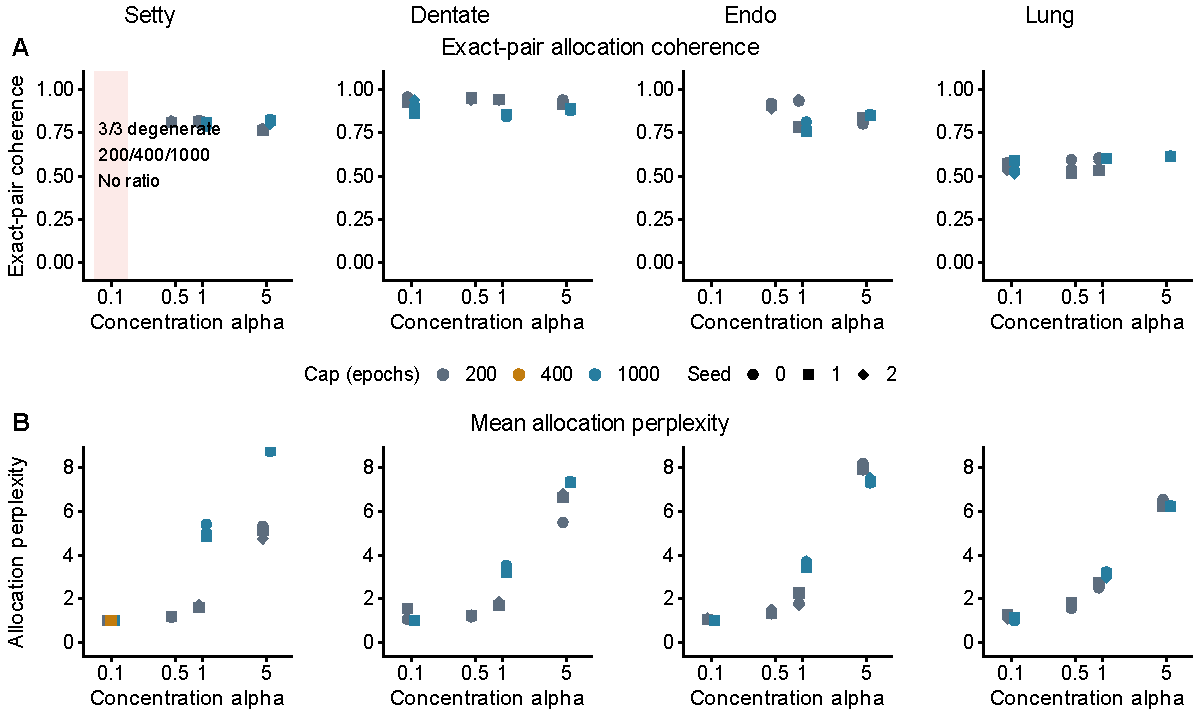
\includegraphics[width=\textwidth,height=0.72\textheight,keepaspectratio]{figures/collapse_alpha.pdf}
\caption{\textbf{Historical concentration and degeneracy across budgets.} Rows A/B show exact-pair coherence/mean perplexity; columns identify backgrounds. Logarithmic $\alpha=0.1,0.5,1,5$ has small budget offsets; $\alpha=2$ is excluded. The inter-row key identifies cap by color and seeds 0--2 by shape. Points are individual endpoints without error bars. The dedicated Setty 400-cap check contributes only $\alpha=0.1$ perplexity. Shading marks three degenerate Setty seeds at each cap, not zero coherence. Caps include early stopping; missing combinations are not a factorial time course.}
\label{fig:collapse}
\end{figure}
\begin{figure}[htbp]
\centering
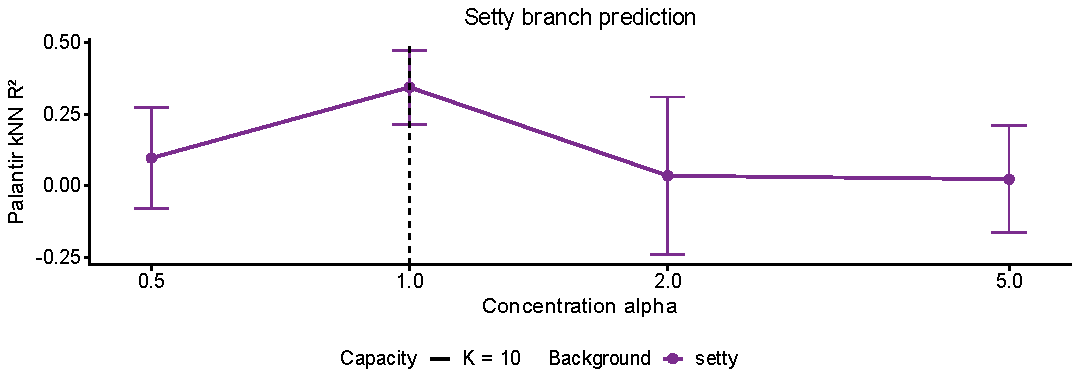
\includegraphics[width=\textwidth,height=0.72\textheight,keepaspectratio]{figures/topic-transformer_branch.pdf}
\caption{\textbf{Historical Setty branch-proxy response, $K=10$, 200-epoch cap.} Five-fold $k$NN $R^2$ predicts stored Palantir branch probabilities against logarithmic concentration. Points/bars are three-seed means/sample SD; the dashed line marks $\alpha=1$. The horizontal key identifies Setty and capacity. Degenerate $\alpha=0.1$ and unreliable summaries are withheld, not assigned zero. Agreement on the fixed within-file split concerns a computed annotation, not observed fate or an attention-specific effect.}
\label{fig:branch}
\end{figure}

\subsection{The failure is not uniform across backgrounds}
At the 1000 cap, Endo $\alpha=0.1$ is degenerate only on seed 0, while the dentate and lung runs remain live. Setty-specific status cannot be generalized to all tissues or all attention encoders. The figure uses only doses shared or explicitly present across the relevant locks, so it is not a complete factorial time course.

\subsection{Two-dimensional purity and Gaussian comparison}
For stored 200-cap Setty coordinates, Corrected purity is $0.355\pm0.021$ at $\alpha=0.1$ and $0.381\pm0.042$ at $\alpha=1$. A visually organized projection or similar label purity does not validate the nearly constant native allocation. Figure~\ref{fig:umap400} and Table~\ref{tab:umappurity400} instead show the $\alpha=1$ 400-cap comparison: topic purity is $0.499\pm0.056$ and control purity is $0.809\pm0.016$. These are stored-label statistics on independent UMAP fits, not evidence that the control recovered a biological lineage.
\begin{figure}[htbp]
\centering
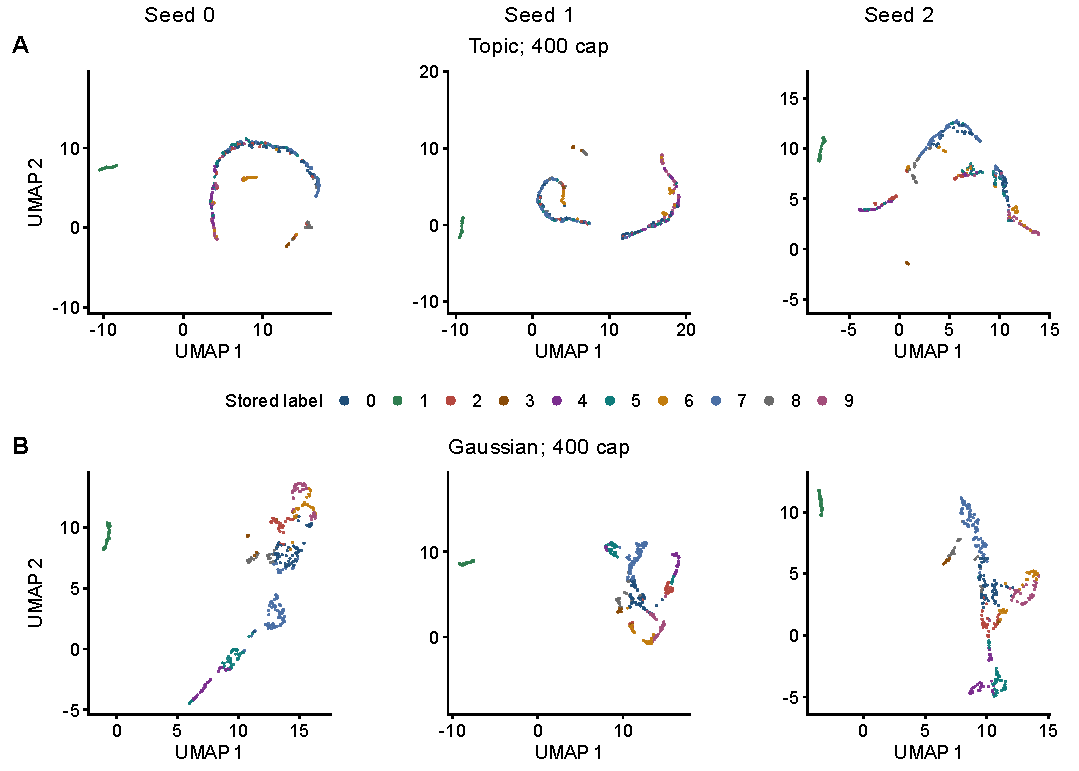
\includegraphics[width=\textwidth,height=0.72\textheight,keepaspectratio]{figures/topic-transformer_setty_umap_400.pdf}
\caption{\textbf{Stored Setty projections at the 400-epoch cap.} Row A: Topic, $\alpha=1$, $K=10$; row B: Gaussian comparator. Columns show seeds 0--2, each retaining 450 held-out cells. The inter-row key preserves ten label codes and common colors. Each UMAP fit is independent, dimensionless and equal-aspect within its tile. Corrected first-15-nonself-neighbor purity changes no coordinates. No cells or seeds are averaged. The comparator differs in geometry, likelihood and decoder; projection shape does not establish lineage recovery.}
\label{fig:umap400}
\end{figure}
\begin{table}[htbp]
\centering
\caption{\textbf{Corrected 400-cap UMAP label purity.} All entries use the first 15 non-self neighbors in the fixed two-dimensional coordinates (version umap-knn15-nonself-v2). This is a label-neighborhood diagnostic, not lineage recovery or a native-latent allocation score.}
\label{tab:umappurity400}
\small
\begin{tabular}{lcccc}
\toprule
Dose & seed 0 & seed 1 & seed 2 & mean $\pm$ s.d. \\
\midrule
$\alpha=1$ & 0.493 & 0.445 & 0.558 & $0.499 \pm 0.056$ \\
control & 0.797 & 0.827 & 0.804 & $0.809 \pm 0.016$ \\
\bottomrule
\end{tabular}

\end{table}

The Gaussian control has different latent geometry, likelihood, decoder and parameter count. Table~\ref{tab:control} reports its historical readouts, but shared seeds and caps do not isolate the prior or attention. At shipped $\alpha=1$, Setty Palantir $k$NN $R^2$ is $0.345\pm0.130$ at 200 epochs and has mean 0.413 at 400, with seed variation. The control has higher scores in these archived comparisons and on each seed at cap 1000. Such ordering is local to the implementation, split and proxy.
\begin{table}[htbp]
\centering
\caption{\textbf{Historical Gaussian-control and topic readouts.} Seeds and cap are aligned but likelihood, decoder, parameter count and latent geometry differ. This is not an attention-only or prior-only ablation. Reachability is shown for context; Palantir scores are computational branch-prediction readouts.}
\label{tab:control}
\small
\setlength{\tabcolsep}{5pt}
\begin{tabular}{llcccc}
\toprule
Quantity & Arm & seed 0 & seed 1 & seed 2 & mean \\
\midrule
\multirow{2}{*}{Setty Palantir $k$NN $R^2$}
 & $\alpha=1$ & 0.202 & 0.377 & 0.455 & 0.345 \\
 & control & 0.476 & 0.814 & 0.692 & 0.661 \\
\midrule
\multirow{2}{*}{Separation survival}
 & $\alpha=1$ & 0.707 & 0.712 & 0.724 & 0.714 \\
 & control & 0.941 & 0.909 & 0.873 & 0.907 \\
\midrule
\multirow{2}{*}{Reachability survival}
 & $\alpha=1$ & 0.841 & 0.838 & 0.838 & 0.839 \\
 & control & 1.000 & 1.000 & 1.000 & 1.000 \\
\bottomrule
\end{tabular}
\end{table}
\begin{table}[htbp]
\centering
\caption{\textbf{400-epoch Setty low-concentration check.} Three topic runs and three Gaussian controls complete 400 epochs. Degenerate topic allocations retain perplexity near one; coherence and branch scores are n.q. because the ratio is degenerate. The control has no native topic allocation.}
\label{tab:alpha0p1400}
\scriptsize
\setlength{\tabcolsep}{3.5pt}
\begin{tabular}{lccccc}
\toprule
Seed & Coherence & Perplexity & Degenerate & Palantir $k$NN $R^2$ & Control Palantir $k$NN $R^2$ \\
\midrule
0 & \textit{n.q.} & 1.000 & yes & \textit{n.q.} & 0.626 \\
1 & \textit{n.q.} & 1.000 & yes & \textit{n.q.} & 0.797 \\
2 & \textit{n.q.} & 1.000 & yes & \textit{n.q.} & 0.765 \\
\bottomrule
\end{tabular}

\end{table}
\begin{table}[htbp]
\centering
\caption{\textbf{Setty rows from the historical 1000-cap transformer subset.} The model-specific archive contains 48 runs across four backgrounds. An asterisk marks early stopping; actual completed epochs are printed per seed. Dashes mark non-native Gaussian allocations. Degenerate coherence and branch readouts are n.q.; the old zero sentinels remain only in immutable archives.}
\label{tab:shipped1000}
\footnotesize
\setlength{\tabcolsep}{2pt}
\begin{tabular}{llcccccc}
\toprule
Arm & Seed & Coherence & Perplexity & Degenerate & Reachability & Palantir $k$NN $R^2$ & Epochs trained \\
\midrule
\multirow{3}{*}{$\alpha=0.1$} & 0 & \textit{n.q.} & 1.000 & yes & 1.000 & \textit{n.q.} & 607$^{\ast}$ \\
 & 1 & \textit{n.q.} & 1.000 & yes & 1.000 & \textit{n.q.} & 492$^{\ast}$ \\
 & 2 & \textit{n.q.} & 1.000 & yes & 1.000 & \textit{n.q.} & 536$^{\ast}$ \\
\midrule
\multirow{3}{*}{$\alpha=1$} & 0 & 0.786 & 5.417 & no & 1.000 & 0.554 & 1000 \\
 & 1 & 0.809 & 4.880 & no & 1.000 & 0.596 & 1000 \\
 & 2 & 0.799 & 5.108 & no & 0.838 & 0.635 & 1000 \\
\midrule
\multirow{3}{*}{Gaussian-latent control} & 0 & --- & --- & --- & 1.000 & 0.752 & 551$^{\ast}$ \\
 & 1 & --- & --- & --- & 0.838 & 0.779 & 698$^{\ast}$ \\
 & 2 & --- & --- & --- & 1.000 & 0.764 & 587$^{\ast}$ \\
\bottomrule
\end{tabular}

\end{table}

\subsection{A repeated graph fraction does not identify a component}
Figure~\ref{fig:tear} shows reachability survival across doses and budgets. The fraction near 0.837664 recurs in several Setty runs, while cap-1000 $\alpha=1$ reachability is 1, 1 and approximately 0.838. The Gaussian control can also tear. Equality of a scalar fraction is insufficient to conclude that the identical edges or component were lost; that requires identity-level graph comparison. Allocation collapse and reachability are distinct diagnostics and need not be ordered together.
\begin{figure}[htbp]
\centering
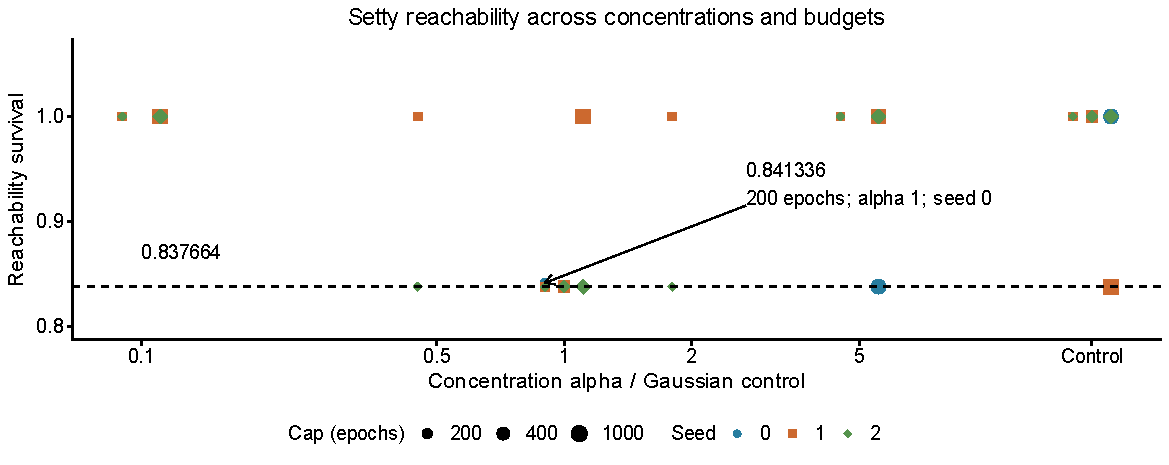
\includegraphics[width=0.92\textwidth,height=0.72\textheight,keepaspectratio]{figures/tear_vs_alpha.pdf}
\caption{\textbf{Setty reachability across historical caps.} The score is the retained fraction of reference-connected cell pairs. Logarithmic concentration has a separate Gaussian-control category and cap-specific offsets. The shared key maps color/shape to seed and size to cap (200, 400, 1000). Each point is an endpoint, without aggregation or error bars. The dashed reference is 0.837664; the annotated 200-cap $\alpha=1$ seed-0 value is 0.841336. Repeated fractions do not identify the same severed component. Near-degenerate graph geometry retains the tie and rounding limitations in Methods.}
\label{fig:tear}
\end{figure}



\subsection{A matched training experiment limits the collapse claim}
All twelve new concentration arms complete 200 epochs, 3200 optimizer updates and 409600 cell presentations. Within each dataset--seed pair, the autoencoder initialization hash and saved batch/random schedule match; concentration-dependent prior buffers intentionally differ. No non-finite update is skipped and no run is selected by its score. Figure~\ref{fig:matched-training} and Table~\ref{tab:matched-training} retain all final states.

The fresh Setty comparison reproduces strict low-concentration collapse on two seeds, not all three. At $\alpha=0.1$, seeds 1 and 2 have maximum coordinate ranges $5.72\times10^{-13}$ and $1.74\times10^{-12}$, respectively; seed 0 has range 0.192837 and therefore fails the prespecified collapse criterion despite mean perplexity 1.002292. All three $\alpha=1$ Setty allocations are nondegenerate. Dentate has no strictly collapsed run at either concentration. In particular, Dentate seed 2 at $\alpha=0.1$ has mean perplexity approximately one but coordinate range one: different cells can occupy different corners. This observation directly demonstrates why within-cell concentration cannot stand in for between-cell collapse. The unfavorable replication for a universal-collapse claim is retained.
\begin{figure}[htbp]
\centering
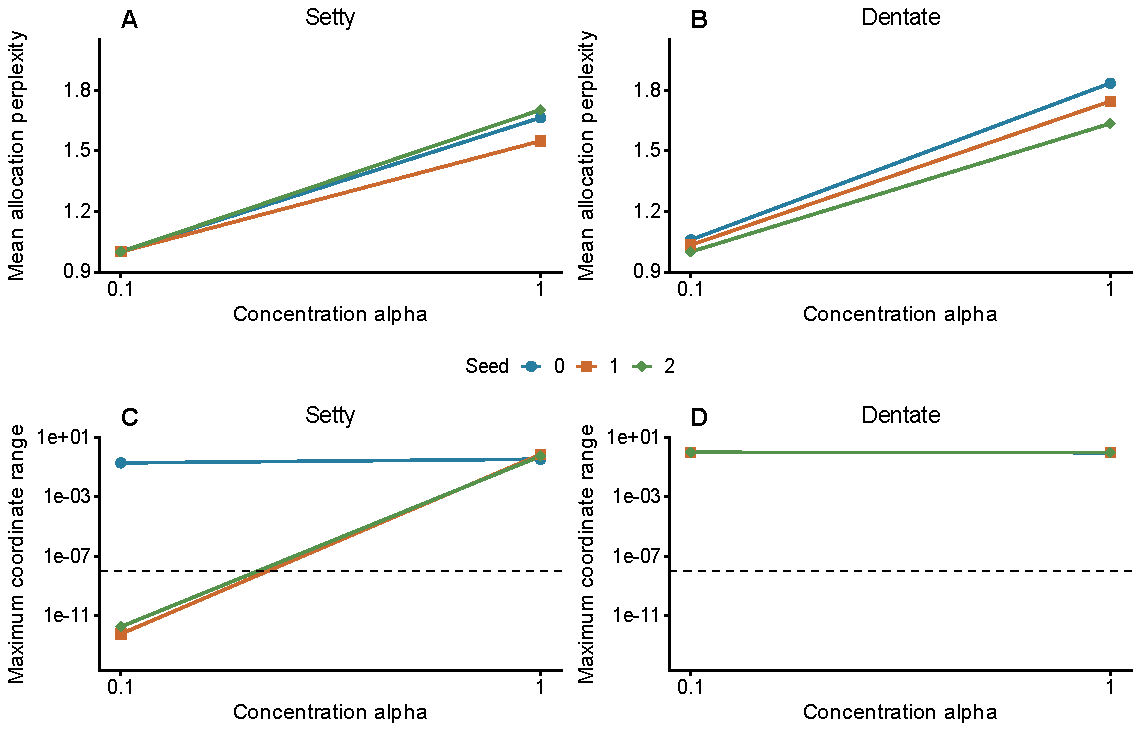
\includegraphics[width=.98\textwidth,height=0.72\textheight,keepaspectratio]{figures/matched_training.pdf}
\caption{\textbf{Matched concentration training.} A/B: Setty/Dentate mean perplexity. C/D: their maximum across-cell coordinate ranges on log scales. Lines join matched $\alpha=0.1$ and 1 endpoints; the inter-row key identifies seeds. Each point summarizes 450 cells, without seed averaging or error bars. All twelve arms complete 3200 updates and 409600 presentations. Strict collapse requires the dashed $10^{-8}$ range threshold and one occupied argmax topic. Perplexity near one alone is insufficient.}
\label{fig:matched-training}
\end{figure}
\begin{table}[htbp]
\centering
\caption{\textbf{All matched-training endpoints.} Range is the maximum over topic coordinates of the across-cell range. Occupancy counts distinct argmax topics. Strict collapse requires range at most $10^{-8}$ and occupancy one. The exact mean distinct-pair Jensen--Shannon divergence determines the separate degeneracy flag. Seed repetitions remain nested in two public data objects.}
\label{tab:matched-training}
\small
\begin{tabular}{llrrrrl}
\toprule
Dataset & Seed / $\alpha$ & Perplexity & Range & Occupancy & Pair JS & Collapse \\
\midrule
Setty & 0 / 0.1 & 1.0023 & 1.93e-01 & 1 & 4.87e-04 & no \\
Setty & 0 / 1 & 1.6640 & 3.45e-01 & 1 & 1.44e-02 & no \\
Setty & 1 / 0.1 & 1.0000 & 5.72e-13 & 1 & 2.39e-16 & yes \\
Setty & 1 / 1 & 1.5485 & 7.16e-01 & 2 & 4.78e-02 & no \\
Setty & 2 / 0.1 & 1.0000 & 1.74e-12 & 1 & 2.20e-15 & yes \\
Setty & 2 / 1 & 1.7029 & 5.54e-01 & 2 & 3.08e-02 & no \\
Dentate & 0 / 0.1 & 1.0591 & 1.00e+00 & 2 & 2.70e-01 & no \\
Dentate & 0 / 1 & 1.8347 & 9.40e-01 & 3 & 1.86e-01 & no \\
Dentate & 1 / 0.1 & 1.0334 & 1.00e+00 & 2 & 2.85e-01 & no \\
Dentate & 1 / 1 & 1.7450 & 9.61e-01 & 3 & 2.44e-01 & no \\
Dentate & 2 / 0.1 & 1.0000 & 1.00e+00 & 2 & 2.83e-01 & no \\
Dentate & 2 / 1 & 1.6351 & 9.65e-01 & 3 & 2.39e-01 & no \\
\bottomrule
\end{tabular}

\end{table}

Independent native-array recomputation confirms Setty $\alpha=0.1$: $2/3$ strict collapse (exact 95\% interval 0.094--0.992); Setty $\alpha=1$ and Dentate at both concentrations: each $0/3$ (0--0.708). All twelve classifications remain unchanged at exploratory range thresholds $10^{-10}$ and $10^{-6}$. Removing Setty seed 0 gives $2/2$ collapsed low-concentration runs, whereas removing seed 1 or 2 gives $1/2$; these are influence checks, not new replications. The seed-0 counterexample therefore remains consequential despite threshold stability. These intervals condition on fixed public objects and do not estimate donor or cohort prevalence. All 144 saved probe summaries also reproduce from their archived allocation arrays within float32 reduction tolerance.

\subsection{Trained-state implementation checks: token sensitivity and batch invariance}
The expected complete-token permutation and batch-context invariances check the implemented within-cell pathway; they are not scientific discoveries or evidence of attention as the cause of collapse.
Figure~\ref{fig:token-probes} tests every trained endpoint under both evaluation and zero-dropout training modes. Reversing complete tokens changes allocations by at most $4.77\times10^{-7}$, below the frozen $10^{-5}$ invariance tolerance. Altering the 48 companion cells or reversing batch order leaves the focal-cell allocations unchanged; isolated-cell evaluation differs by at most $9.84\times10^{-7}$. Thus these probes do not detect cross-cell mixing in the implemented deterministic encoder.

Content-changing interventions have a different response. Replacing all tokens by their per-cell mean gives an overall mean allocation $L_1$ change of 0.074070, while duplicating the first complete token gives 0.148893; individual coordinate changes can reach one. These averages combine the twelve endpoint states and two execution modes solely to describe probe magnitude, not independent biological replication. The per-state plot retains the heterogeneous responses. The result establishes sensitivity to token content in parts of the trained system, while providing no unique explanation of why two particular low-concentration runs collapsed.
\begin{figure}[htbp]
\centering
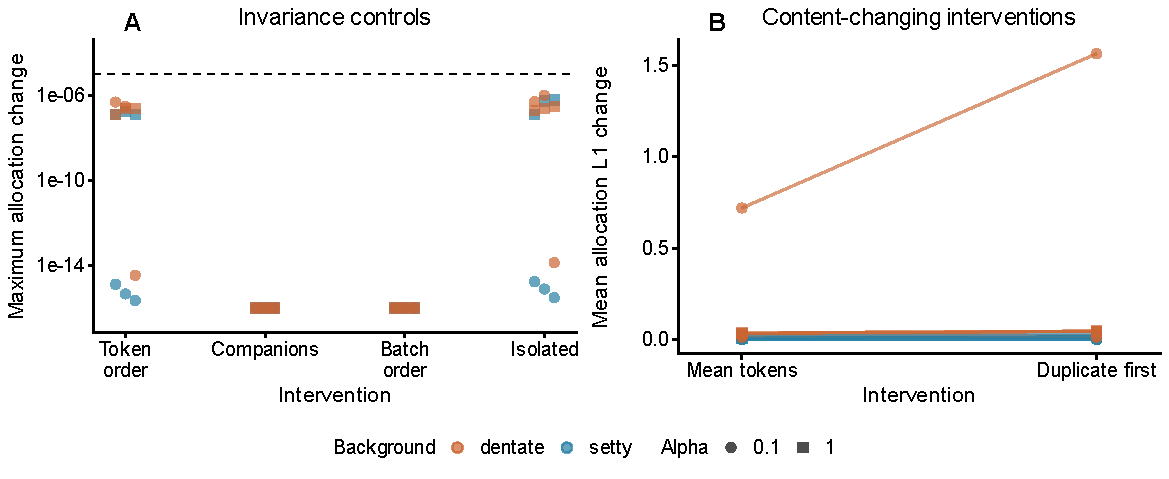
\includegraphics[width=.98\textwidth,height=0.72\textheight,keepaspectratio]{figures/token_probes.pdf}
\caption{\textbf{Trained-state token interventions.} A: maximum allocation change for token reversal, altered companions, restored batch reversal and isolated evaluation (log scale; values below $10^{-16}$ displayed at that floor). The dashed line marks the frozen $10^{-5}$ tolerance. B: mean row $L_1$ change under mean-token replacement and first-token duplication; lines join each state. Color/shape identify background/concentration. All twelve evaluation-mode states are retained without seed averaging or error bars. Probes use 64 test cells and 16 focal cells for context controls, with zero updates; training-mode probes use zero dropout.}
\label{fig:token-probes}
\end{figure}

\section{Discussion}
The matched Setty low-concentration strict-collapse rate is $2/3$ (exact 95\% interval 0.094--0.992); each other matched cell is $0/3$ (0--0.708). Three seeds cannot locate collapse probability precisely. The parameter-matched MLP gate and 20-or-more new seeds per complete phase-diagram cell remain unexecuted. Comparable MLP collapse or failure of the proposed discordance gate would preclude attention-specific framing. The native arrays establish a narrower failure: a valid simplex can retain probability mass and tiny nonzero tails while losing almost all between-cell variation. Dominant topic identity may differ across seeds.

Historical degeneracy at the 200 endpoint, after 400 complete epochs and after longer-cap early stopping makes a purely short-budget failure less plausible. These endpoints nevertheless differ in exposure and random trajectory. The fresh comparison matches initialization, minibatches, stochastic draws and updates, varying concentration-dependent prior buffers. Its noncollapsed Setty seed and all noncollapsed Dentate arms prevent a universal low-concentration claim. Range-threshold stability does not remove seed influence or provide additional replication.

The trained-state probes test a different question. Complete-token permutation with embeddings attached and changes to companion cells check the intended computational axes; token homogenization and duplication test content sensitivity. Their observed invariances and heterogeneous changes describe this deterministic encoder. They neither identify why training reached a particular allocation nor assign biological meaning to a changed projection. The tokens are full-expression projections, so they cannot be interpreted directly as named gene programs.

The exact objective also narrows mechanistic interpretation. The custom shortfall penalty reverses the low-KL derivative instead of implementing a flat free-bits allowance. The decoder uses normalized count cross-entropy, and the prior is a diagonal logit-space surrogate. These choices remain potential contributors alongside attention. No ablation separates their effects, and constancy of the exported posterior mean after softmax does not establish equality of the full posterior and prior. An attention-versus-MLP comparison must hold these objective and optimization choices fixed.

Measurement status must precede interpretation. Exact-pair coherence is still undefined when its denominator vanishes; a zero sentinel cannot measure biological incoherence. Corrected UMAP purity leaves coordinates unchanged and cannot rescue a collapsed native allocation. The archived graph helper also assumes the first neighbour is self: an exact-duplicate stress case retains self-loops. Although the twelve new arrays have no exact cutoff ties, very small distances and untested rounding sensitivity limit near-collapsed geometry. A repeated reachability fraction cannot identify the same lost edges or component.

Palantir~\cite{setty2019palantir} prediction measures agreement with a computed annotation, not lineage tracing. The Gaussian comparator changes geometry, likelihood, decoder and parameter count simultaneously; its higher contextual scores cannot isolate attention or prior effects. Mixed off-Setty behavior further restricts the claim to the observed configuration and fixed public objects.

Feature selection precedes splitting and the expression graph is transductive. Repeated optimization seeds therefore estimate neither independent-donor variability nor inductive transfer. No experiment intervenes on a decoded gene program or validates a clinical prediction. Subsequent biological use requires a useful native representation, a matched encoder control and independent-sample evaluation before interpreting topic proportions or attention as biological evidence.

\FloatBarrier
\section{Declarations}
\noindent\textbf{Data and code availability}\par\nobreak
The study-specific source repository is \url{https://github.com/PeterPonyu/attention-topic-collapse}; the versioned research archive is \url{https://doi.org/10.5281/zenodo.22914481}. The archive contains the manuscript, vector figures, matched training and intervention records, saved allocation arrays, schedules, protocols and source snapshots. CPU commands reproduce collapse intervals and saved-result numerical diagnostics without training, source-expression snapshots or model checkpoints. Model checkpoints are supplied separately within this archive. Processed Setty and Dentate source-expression snapshots are not distributed because their exact upstream-version and annotation-transformation provenance has not been established for redistribution. Historical model-state probes and training additionally require separately and lawfully obtained, hash-matching expression inputs. Raw-data preprocessing, every historical training sweep and graph-score regeneration are outside the verified public reproduction scope. The repository README gives the dependency requirements, commands and checksums. Source studies and their data-access conditions are identified in Materials and Methods and the bibliography. Author-owned software is MIT licensed; the author's manuscript, figures, generated results and weights are CC BY 4.0. Third-party data and annotations retain their original terms.

\noindent\textbf{Ethics approval and consent}\par\nobreak

This study reuses the public expression datasets identified in Materials and Methods. The manuscript reports computational analyses of existing data. Author confirmation of any ethics review or exemption applicable to this secondary analysis, the original consent conditions, and consent for publication has not been established in this report. No new approval or exemption is asserted here.

\noindent\textbf{Funding}\par\nobreak

This research received no funding.

\noindent\textbf{Author contributions}\par\nobreak

Zeyu Fu is the sole author and is responsible for this manuscript.

\noindent\textbf{Competing interests}\par\nobreak
The author declares no competing interests.

\bibliographystyle{plainnat}
\bibliography{standalone-assets/refs,extra}
\end{document}
